\chapter{Radar simulation with Vulkan}\label{ch:method}

% This chapter describes the core of your work: the methodology you used to solve the problem
% you described in the Introduction. It is quite likely to have a different name (e.g., the
% name of the tool you wrote), and/or to be split into multiple chapters. It will likely be quite
% densely connected with things you have written in the Background chapter (\Cref{sec:background}),
% and the results that you will show in the Results chapter (\Cref{sec:results}). Put abundant
% references to help the reader navigate the document.
%
% Try to keep a level of detail such that a skilled reader will be able to reproduce your result,
% but do not include unnecessary details that the reader can find out for themselves (e.g., the
% list of commands to perform a standard task). That is indeed valuable information that can help
% reproducibility, but if you do not think it is needed to understand your work, its place is
% likely to be in an appendix or in the documentation of the code you wrote, if you decide to
% release it.
%
% This chapter should include work that has been done by you. If that is not the case, consider
% moving it to the Background chapter (\Cref{sec:background}), or make it very clear that you are
% not the author. The same thing applies to images: if they aren't yours, you should cite the
% source.
%
% The results of your work should generally not be included in this chapter. In some cases,
% preliminary results can be included to explain why you took a certain direction in your work
% (e.g., you took a choice rather than another because you measured that it was more efficient),
% but the overall evaluation of your work should be in the Results chapter (\Cref{sec:results}).
%
% You are likely to include algorithms in pseudocode. Check
% \href{https://www.overleaf.com/learn/latex/Algorithms}{relevant \latex packages} for that.

In this chapter we present our radar simulator, implemented using the
Vulkan ray tracing pipeline
(\autoref{subsec:raytracing}) and
the Rust programming language. Our simulator is based on the \emph{shooting and
bouncing ray} (SBR) method. In particular, we use the probabilistic approach 
presented by Schüßler et al.~\cite{mimo}.

In the following sections we present a detailed description of each
of the building blocks the simulator consists of.

\section{Simulation of the transmitting antenna and ray
generation}\label{sec:myraygen}

The transmission by the radar antenna is simulated by the casting of rays. Those rays are 
generated by a ray generation shader
(\autoref{subsubsec:raygen}).
A configurable number $N_{\text{TX}}$ of rays is generated, each with the same
power simply given by dividing the radar transmitting power $\powradiated$ by
the number of rays. The direction of the rays is randomly chosen based on the
directivity of the antenna, in particular, we use the following probability density
function:
\begin{equation}\label{eq:pdf}
	pdf(\theta, \phi) = \frac{1}{4\pi}D(\theta, \phi) \sin\theta d\theta d\phi 
\end{equation}
where $D(\theta, \phi)$ is the directivity of the transmitting antenna.

\begin{remark}
	\autoref{eq:pdf} is a valid probability density function, i.e.:\begin{equation}
		\int_0^{2\pi}\int_0^\pi \frac{1}{4\pi}D(\theta, \phi) \sin\theta d\theta d\phi = 1
	\end{equation}
\end{remark}
\begin{proof}
	Obvious from \autoref{eq:directivity} and \autoref{eq:radiationintensity}.
\end{proof}

Considering now a solid angle $\omega$, we verify that the expected power
generated in it is equal to the actual power the antenna with the given
directivity radiates there. First we compute the probability $p_\omega$ that 
a ray's direction is chosen in $\omega$:
\begin{equation}\label{probregion}
	p_\omega = \frac{1}{4\pi}\iint_\omega D(\theta, \phi) \sin\theta d\theta d\phi
\end{equation}
The probability of generating $k$ rays in $\omega$ from a total of
$N_\text{TX}$ rays is described by the binomial random variable $N_\omega$:
\begin{equation}
	Pr\left(N_\omega = k \right) = \binom{N_\text{TX}}{k} p_\omega^{k} (1-p_\omega)^{N_\text{TX} - k}
\end{equation}
Since to each ray is associated the same power $\powradiated/N_\text{TX}$, we can define the 
random variable $P_\omega$, describing the total power which is randomly chosen to be 
radiated in $\omega$, simply as:
\begin{equation}
	P_\omega = \frac{\powradiated}{N_\text{TX}} N_\omega
\end{equation}
The following remark shows that the expected value of $P_\omega$ is equal to the actual power 
an antenna would radiate in $\omega$.

\begin{remark}
\begin{equation}
	\mathbb{E}\left[P_\omega\right] = \iint_\omega U(\theta, \phi) \sin \theta d\theta d\phi
\end{equation}
\end{remark}
\begin{proof}
\begin{align}
	\mathbb{E}\left[P_\omega\right] &= 
	\mathbb{E}\left[\frac{\powradiated}{N_\text{TX}}N_\omega\right] =\\
	&= \frac{\powradiated}{N_\text{TX}}\mathbb{E}\left[N_\omega\right] =\\
	&= \frac{\powradiated}{N_\text{TX}}N_\text{TX}p_\omega = \\
	&= \powradiated p_\omega =\\
	&= \powradiated \frac{1}{4\pi}\iint_\omega D(\theta, \phi) \sin\theta d\theta d\phi =\\
	&= \powradiated \frac{1}{4\pi}\iint_\omega \frac{U(\theta, \phi)}{\powradiated / (4\pi)} \sin\theta d\theta d\phi =\\
	&= \iint_\omega U(\theta, \phi) \sin\theta d\theta d\phi
\end{align}
\end{proof}

In general, the directivity of an antenna, and therefore the $pdf$ in
\autoref{eq:pdf},  are not known as an analytic expression, 
but only in a finite set of points, either from real world measurement or 
from numerical computations. For this reason, our simulator parametrizes the
antenna directivity as a 2D texture over spherical coordinates. Each 
point $D_{i,j}$ in the texture is the value of the directivity
at the direction, in spherical coordinates, given by:
\begin{equation}\label{eq:ij-dir}
	(i \frac{\pi}{D_\text{zenith}}, j \frac{2\pi}{D_\text{azimuth}})
\end{equation}
where $D_\text{azimuth}$ is the resolution in azimuth and $D_\text{zenith}$ is
the resolution in zenith of the texture. To each point in the texture we
associate a region where we assume constant directivity (the error from this
approximation can be decreased by increasing the resolution) centered around
the direction given by \autoref{eq:ij-dir} and defined by 
\begin{gather}
	\theta \in [(i - \frac{1}{2})\frac{\pi}{D_\text{zenith}}, (i + \frac{1}{2})\frac{\pi}{D_\text{zenith}}  ] \\
	\phi \in [(j - \frac{1}{2})\frac{2\pi}{D_\text{azimuth}}, (j + \frac{1}{2})\frac{2\pi}{D_\text{azimuth}}  ]
\end{gather}

The probability for a ray to be generated in one region is given by
\autoref{probregion} but, since we assumed the directivity to be constant over
the region, it is given simply by multiplying the directivity $D_{i,j}$ with
the area of the region. The problem of randomly choosing the direction for a
ray using the probability density function in \autoref{eq:pdf}
can now be reformulated as the problem of sampling from a discrete distribution
which selects one of the points in the directivity texture. This can be
achieved efficiently using the alias method \cite{Walker1974NewFM}.
Once a point in texture has been selected, the corresponding direction is
computed using \autoref{eq:ij-dir} and displaced in azimuth
and zenith by a random amount.

The advantage of generating rays using a probability density function based on
the directivity of the antenna, as opposed to generating rays uniformly in all
directions as done by Schüßler et al.~\cite{mimo}, is that we can have a much
higher density of rays where the directivity is high, saving computational time
where the directivity is low as the tracing of rays there would not significantly
change the result of the simulation. Having a greater number of rays in
the main lobe, in turn, allows for the detection of smaller or farther targets.

Apart from choosing the initial ray direction as described to simulate the
transmitting antenna, the ray generation shader also iteratively traces the
rays resulting from the interaction with objects in the scene. This is done as
shown in \autoref{code:raygen}, by using the direction the closest-hit shader
has written in the ray payload. The origin of the ray is updated to the point
of intersection with the object. The tracing terminates when either the power
falls under a configurable cutoff or the maximum number of bounces is reached.
The payload, associated to each ray, is defined by the structure in
\autoref{code:ray-payload}. This payload contains the power associated with the
ray, as well the distance it has travelled so far, the doppler shift it has
been subject of, the output direction of the closest-hit and finally the
parameter $t$ which indicates the distance the ray has travelled from the
origin to the intersection.

\begin{listing}
	\begin{minted}{glsl}
vec3 direction = gen_direction(transmitter, rng_state, directivity);
uint rayFlags = gl_RayFlagsOpaqueEXT;
uint cullMask = 0xff;
float tmin = 0.01;
float tmax = 10000.0;
for (int i = 0; i < MAX_DEPTH && payload.power > transmitter.cutoff; i++) {
	traceRayEXT(
		topLevelAS,
		rayFlags,
		cullMask,
		0, 0, 0,
		origin,
		tmin,
		direction,
		tmax,
		0
	);
	origin += payload.t * direction;
	direction = payload.outDir;
}
	\end{minted}
	\caption{The ray generation code that iteretatively traces the initial ray
	originating from the transmitter and its bounces. The direction for the
	subsequent rays is obtained from the closest-hit shader, as outputted in
	the ray payload. The origin for the new ray is obtained by advancing from
	the origin along the direction by the parameter \texttt{t}, also given by
	the closest-hit shader. The \texttt{gl\_RayFlagsOpaqueEXT} flag skips the
	any-hit shader, since we do not use it.}
	\label{code:raygen}
\end{listing}

\begin{listing}
	\begin{minted}{glsl}
struct RayPayload {
	float power;
	float distance;
	float shift_freq;
	vec3 outDir;
	float t;
};
	\end{minted}
	\caption{The ray payload associated with each ray.}
	\label{code:ray-payload}
\end{listing}

\section{Targets and Environment Modeling}

The targets and the environment are simulated as multiple triangle meshes. 
Each mesh is associated with the information required for the simulation:
\begin{itemize}
	\item a three dimensional vector indicating its position;
	\item a scalar, used to scale the mesh;
	\item a quaternion, representing its rotation;
	\item a three dimensional vector specifying the velocity of the object;
	\item a three dimensional vector encoding its angular velocity;
	\item a material identifier, which specifies which shader to use when the
		mesh is hit by a ray
		(\autoref{sec:materials}). This identifier is 
		a 24-bit number used as \texttt{instanceShaderBindingTableRecordOffset}
		field in the structure \texttt{VkAccelerationStructureInstanceKHR} so that the right
		closest-hit shader, implementing the material, is automatically called during the acceleration
		structure traversal (\autoref{subsec:sbt}).
\end{itemize}
In order to use a mesh within the Vulkan ray tracing pipeline, the mesh 
must be added to an acceleration structure. This is done by building a bottom
level acceleration structure (BLAS) for each of the meshes, and then build
the top level acceleration structure (TLAS) out of all the BLAS. When adding
a BLAS to a TLAS, a transformation matrix can be specified. We leveraged this
matrix to encode into the acceleration structure the position, scale and
rotation of each the meshes. In particular the matrix $M_\text{obj}$
associated with an object is given by:
\begin{equation}
	M_\text{obj} = M_\text{translate} \cdot M_\text{scale} \cdot M_\text{rotation}
\end{equation}
where $M_\text{translate}$, $M_\text{scale}$ and $M_\text{rotation}$ are 4 by 4
matrices which respectively translate the object at its position, scale it by a
factor and rotate it. At each step of the simulation, position and rotation are 
updated using respectively the velocity and angular velocity associated with the 
object. Thus, the $M_\text{translate}$ and $M_\text{rotation}$ matrices
are recomputed at every step of the simulation with the updated
position and rotation. After computing the matrices of all the object in the
scene, the TLAS is updated if no new object has been added or otherwise
rebuilt.


\section{Materials}\label{sec:materials}

Each material is modeled as a closest hit shader
(\autoref{subsubsec:closesthitshader}).
At an high-level, there are computations common to all the shaders used
for the modeling of the materials:
\begin{itemize}
	\item compute the reflected direction of the ray after hitting the object. In case the 
		material radiates in multiple directions, such as for a diffusing material, 
		the shader uses a probabilistic model to choose one. This prevents the number
		of rays from growing exponentially with each subsequent bounce;
	\item compute the shift in frequency caused by the doppler effect;
	\item adjust the power associated with the ray, accounting for material
		absorption;
	\item adjust the distance the ray traveled, used for the delay computation.
\end{itemize}
In order to perform those computations, the shader is provided with an array of
structures, one for each mesh in the acceleration structure, containing the
geometry information, in the form of a index buffer and vertex buffer, and
velocity and angular velocity vectors. The type of the element of this array is
the structure \texttt{ObjectInfo} shown in \autoref{code:object-info}. The
fields \verb!v_buf! and \verb!i_buf! contain the device address of the buffer
containing the vertices and indices, respectively. In order to use pointers in
this way in GLSL it is necessary to enable the extension
\verb!GLSL_EXT_buffer_reference! \cite{buffer-reference}.

\begin{listing}
	\begin{minted}{glsl}
layout(buffer_reference, buffer_reference_align = 8) readonly buffer Vertices {
	Vertex v[];
};
layout(buffer_reference, buffer_reference_align = 8) readonly buffer Indices {
	uint i[];
};
struct ObjectInfo {
	Vertices v_buf;
	Indices i_buf;
	vec3 position;
	float param1;
	vec3 velocity;
	float param2;
	vec3 angular_velocity; 
	float param3;
	float param4;
};
	\end{minted}
	\caption{The structure containing the information associated to each object
	in the scene available to the closest-hit shaders used to implement
	materials. \texttt{params1}, \texttt{params2}, \texttt{params3} and
	\texttt{params4} can be used by the shader to parametrize the behaviour of
	the shader, for example accepting the permittivity and conductivity of the
	material. The reason those parameters are interleaved with \texttt{vec3} is
	to be memory efficient: \texttt{vec3} is 12 bytes in size but is 16 bytes
	aligned, meaning that placing two fields of type \texttt{vec3} next to each
	other would result in a padding of 4 bytes being automatically inserted by
	the compiler to ensure proper alignment. By placing the parameters there we
	can avoid this space to be wasted.}
	\label{code:object-info}
\end{listing}

This array is indexed with the variable
\verb!gl_InstanceID! to find the information relevant to the object hit by the
current ray. The shader then determines the intersection point of the ray with
the mesh and the surface normal there. Those operations are performed by
accessing the vertex buffer, which stores the position of each vertex and its
normal, and interpolating them using barycentric coordinates. After having
determined the point of intersection $P$, the shader computes the tangent 
velocity $\vec v_h$ with \cite{scalabledigitaltwins};
\begin{equation}\label{eq:tangent-velocity}
	\vec v_h = \vec v_0 + \vec\omega \times \vec{OP}
\end{equation}
where $\vec v_0$ is the velocity vector, $\vec\omega$ is the tangent velocity
vector and $\vec{OP}$ is the vector pointing from the origin of the object to
the intersection point. Once the tangent velocity is determined, the doppler
shift is computed. An object which receives an EM wave and then reradiates it
is modeled first as an observer for the reception, and as a source for the
emission. Therefore, we first compute a doppler shift $\Delta_1$ accounting
for the reception:
\begin{equation}\label{eq:doppler-in}
	\Delta_1 = \frac{c - \vec v_h \cdot \vec d_\text{in} }{c}
\end{equation}
where $\vec d_\text{in}$ is the (unit) vector of the direction of the incoming ray
and $\vec v_h$ is the tangent velocity as given by \autoref{eq:tangent-velocity}. The dot
product $\vec v_h \cdot \vec d_\text{in}$ computes the speed along the
direction of the ray and the sign ensures that if the object is moving away
from the source the frequency decreases and if it is moving instead towards the
source the frequency increases. Thus, the frequency $f'$ in frequency-dependant
computations in the shader is given by:
\begin{equation}
	f' = \Delta_1 \cdot f_0
\end{equation}
where $f_0$ is the original frequency. After the output direction of the reflection
$\vec d_\text{out}$ is determined in a per-shader dependant way, then the
Doppler shift $\Delta_2$ accounting for the emission can be computed:
\begin{equation}\label{eq:doppler-out}
	\Delta_2 = \frac{c}{c - \vec v_h \cdot \vec d_\text{out} }
\end{equation}
The frequency $f''$ resulted from both the shifts is thus given by
\begin{equation}
	f'' = \Delta_1 \cdot \Delta_2 \cdot f_0
\end{equation}

We implemented the following different materials based on different physical phenomenons:
\begin{itemize}
	\item a perfectly specular material, which simply reflects the incoming ray
		with no loss of power in the direction specular to the normal of the
		surface. This material models the behaviour of a perfectly conducing
		material. This shader ignores the parameters.
	\item a specular material, which reflects the incoming ray in the direction
		specular to the normal of the surface and adjust its power according to
		the Fresnel equations (\autoref{eq:fresnel}). The effect of
		transmission is not simulated. This shader interprets \texttt{param1}
		as a real index of refraction.
	\item a specular material with transmission. This material computes the reflected
		power and uses it as a probability to either reflect the ray or transmit it. This shader 
		also interprets \texttt{param1} as a real index of refraction.
	\item a specular material with non-zero conductivity. This shader
		interprets the parameters as the parameters of the model presented in
		\autoref{subsub:prop-fit}. Thus, it uses the parameters to compute a
		complex index of refraction and the reflectivity with the Fresnel
		equations.
	\item a diffuse material, which models a rough surface which reflects the
		incoming ray uniformly in the hemisphere around the surface normal.
		This is done by randomly sampling a direction. \texttt{param1} is used
		to model how much absorption the material has, with 1 meaning no power
		is loss and 0 all power is absorbed.
	\item retroreflector. This material reflect the ray in the same but
		opposite direction with respect to the incoming one. This material
		model the behaviour of a corner reflector. While a corner reflector 
		could be modeled with a mesh, a shader does not require to reflect
		the ray multiple times and can therefore be more efficient.
		\texttt{param1} is interpreted as for the diffuse material.
\end{itemize}


\section{Simulation of the receiving antenna}

The receiving antenna is simulated with a reception sphere centered at the
receiver's location. Unlike the targets and simulated environment which are made
of triangle meshes, reception spheres are modeled using an intersection 
shader
(\autoref{subsub:intersectionshader})
and a closest hit shader.
This is more efficient and precise than approximating the sphere surface with
triangles, since we do not need to store a high number of vertices but just 
the center of the sphere and its radius. The sphere is enclosed in an axis
aligned bounding box (AABB) which is inserted in the acceleration structure. In
this way, during ray tracing, if a ray intersects the AABB the intersection
shader is called which will determine if the ray also hits the sphere by
solving the system of equations:
\begin{equation}
	\begin{cases}
		\lVert \vec x - \vec c \rVert^2 = r^2 \\
		\vec x = \vec o + t \vec d
	\end{cases}
\end{equation}
where $\vec c$ is the center of the sphere, $r$ is its radius, $\vec o$ is the
origin of the ray, $\vec d$ is the ray direction and $t$ is parameter of 
the line. If a solution to the system of equations exists, the ray intersects
the sphere and therefore the intersection is reported. If the intersection
is determined to be the closest, the closest hit shader associated with 
the reception sphere is called. In this closest hit shader, first we compute
the contribute of the new received ray to the power density in the area around
the receiving antenna by dividing the power associated with the ray by the area
of the cross section of the sphere, i.e.~the circle with the radius equal to
the radius of the sphere. In this shader, the effective area of the receiving
antenna is computed using \autoref{eq:effectivearea} which requires the gain
and the wave length. The gain is computed by converting the direction of the
incoming ray in spherical coordinates and by using those to sample a texture
containing the gain. The wave length is simply computed from the frequency
(\autoref{eq:wavelength}). Finally the reception sphere's closest hit shader
outputs the power, frequency and distance travelled associated with the ray to
a buffer. The buffer is big enough to accomodate all the generated rays but, in
practice, only a small portion of them will ever be received. For this reason,
the number of received rays is kept as a counter, incremented atomically and
used to place the data of a new received ray continuously in memory. In this
way it is possible to efficiently find the rays which have been received,
without iterating the whole buffer. The received rays, stored in device memory,
are then transferred to the host with the use of a dedicated transfer queue.
The host in turn, write the result to a file or pipe.


\section{Radar simulator as a library and its architecture}\label{sec:architecture}


Our radar simulator is designed to be able to modify the scene at any point
during the simulation. In particular, it is possible to add objects, specifying
models as \texttt{obj} files, their initial position, rotation, velocity and
angular velocity and a material. While at each step of the simulation the
objects position and rotation are updated using velocity and angular velocity,
they can also be updated manually at any point in time. Objects can also be
removed. All those operations can be performed with a particular JSON object.
Our radar simulator accepts as command line argument the path of a file or
named pipe which is read line by line, each line parsed as a JSON object and
the corresponding operation performed. In order to avoid blocking the
simulation when reading from the file, a dedicated thread is run which
continuously read and parse the input. The input command, parsed and validated,
is then either sent to the main thread, when the operation is not costly and
can be performed in the main thread without stalling the simulation, or to a
second thread, which we call loader thread, that handles it. Communication between
those threads happen with the multiple producers single consumer channels from 
the Rust standard library \cite{mpsc}.
Operations we deem costly are the loading of a new object in the scene, which
requires the reading of the \texttt{obj} file from disk and the building of a
new bottom level acceleration structure, the addition of the transmitting
antenna, which requires the initialization of the table needed by the alias
method used for the ray generation (see \autoref{sec:myraygen}) and
transferring it to the device, and the addition of a receiving antenna which
requires to read from disk the texture used for the gain which, once again, is
transferred to the device.

While our current implementation does not support multiple transmitting or
multiple receiving antennas, and therefore the addition of the transmitting and
receiving antennas could be handled before starting the simulation, we still
perform them in the loader thread to facilitate a possible future extension to
add support for multiple transmitting and receiving antennas.

As argument of the program, apart from the already mentioned path of the input
file, our simulator takes the path of an output file or named pipe, to which
the output of the simulation is written at the end of each step. The ability
to accept commands that define and alter the state of the simulation, together
with the ability to yield the output of the simulation continuously, allow our
radar simulator to communicate with other programs, effectively allowing it
to be integrated in other systems. \autoref{fig:architecture} summarizes the
architecture of our radar simulator and its ability to communicate with other
programs.

\begin{figure}\centering
	\begin{tikzpicture}[node distance=2cm]
		\node (external) [anchor=center, rectangle, fill=red!30, draw, minimum height = 2cm] {External program};
		\node (simulator) [matrix, right=6cm of external, draw, fill=blue!20, rounded
			corners, align=right,
			label=above:Radar simulator, anchor=center, nodes=draw, row sep=1cm] {
				\node (parser) [fill=white, minimum width=3cm, minimum height=1cm] {Input thread};
				\node (loader) [fill=white, minimum width=3cm, minimum height=1cm, right=of parser] {Loader thread}; \\
				\node (main)   [fill=white, minimum width=3cm, minimum height=1cm] {Main thread}; \\
			};
		\draw [arrow] (external) -- (parser) node [midway, above] {Pipe};
		\draw [arrow] (main) -- (external) node [midway, above] {Pipe};
		\draw [arrow] (parser) -- (loader) node [midway, above] {MPSC};
		\draw [arrow] (loader) -- (main) node [midway, below] {MPSC};
		\draw [arrow] (parser) -- (main) node [midway, right] {MPSC};
	\end{tikzpicture}
	\caption{Radar simulator architecture. Communication with an external program happens 
	through serialized JSON objects sent trough a pipe. The input thread parses them and forwards
	them to either the loader thread or the main thread. The main thread writes
	the output of the simulation at every step of the simulation, making it
	available to the external program.}
	\label{fig:architecture}
\end{figure}

As previously mentioned, our radar simulator operates in steps and for each of
those step produces an output, containing the rays, which is outputted in the
file/pipe at the specified path. Each step or frame requires co-operation of
both CPU and GPU. In particular, before the GPU can start the ray tracing,
the CPU first must:
\begin{itemize}
	\item check for new commands from the input and loader threads and in case 
		perform the associated action;
	\item update the scene, i.e.~update position and rotation of each and every objects using
		the associated velocity and angular velocity;
	\item record a Vulkan command buffer for the GPU;
	\item finally, submit the command buffer so that the GPU can start working on the step.
\end{itemize}
After the GPU finishes the ray tracing and the transfer of the output buffer,
the CPU must write the content of the output buffer to the file/buffer. Thus,
each step of the simulation requires work from both the CPU and the GPU of the
system and therefore some kind of synchronization among them. A simple but
suboptimal approach would be to have the CPU simply wait for the GPU to
finish. With this configuration, the CPU would remain unutilized when the GPU
works as well the other way around. This would limit the throughput, in steps per
second, to $1/(t_c + t_g)$ where $t_c$ is the average CPU time and $t_g$ is the
average GPU time required for each frame. Thus, in order to maximize the
throughput which the simulator can produce its output at, our implementation
overlaps the work performed by CPU and GPU so that potentially they are always 
utilized. This allows for the throughput to increase to $1/\max{\{t_c, t_g\}}$.
In the best case scenario, when the CPU time $t_c$ and GPU time $t_g$ are
equals, this means the number of steps per second doubles. This technique
is referred to as \emph{frames in flight} \cite{frames-in-flight} and it is
depicted in \autoref{fig:timeline-optimal} for the case where the CPU and GPU
times are equal, and in \autoref{fig:timeline-suboptimal} for the case where
they are not.

\tikzstyle{timeline} = [matrix,
	ampersand replacement=\&,
	row sep=.1cm,
	nodes={minimum width=2cm, minimum height=.7cm, right},
	every odd row/.style={nodes={fill=gray!10}},
	every even row/.style={nodes={fill=gray!40}},
	]
\begin{figure}\centering
	\let\cputimeline=\empty
	\foreach \x in {1,...,3} {
		\xappto{\cputimeline}{
			\noexpand\node [draw, fill=green!30] {\x}; \& \noexpand\node{}; \&
		}
	}
	\let\gputimeline=\empty
	\foreach \x in {1,...,3} {
		\xappto{\gputimeline}{
			\noexpand\node{}; \& \noexpand\node [draw, fill=blue!30] {\x}; \&
		}
	}
	\begin{subfigure}[t]{\textwidth}\centering
		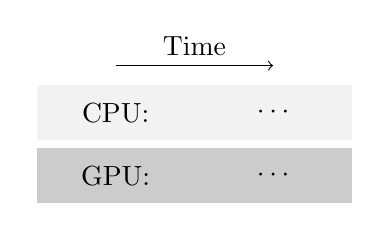
\begin{tikzpicture}
			\draw[->] (-1, 1) -- (1, 1) node [midway, above] {Time};
			\matrix (timeline) [timeline] {
				\node {CPU:}; \& \cputimeline ; \node {$\cdots$}; \\
				\node {GPU:}; \& \gputimeline ; \node {$\cdots$}; \\
			};
		\end{tikzpicture}
		\subcaption{Execution time line for one frame in flight.}
	\end{subfigure}
	\undef\cputimeline
	\undef\gputimeline

	\let\cputimeline=\empty
	\foreach \x in {1,...,5} {
		\xappto{\cputimeline}{
			\noexpand\node [draw, fill=green!30, minimum width=2cm] {\x}; \&
		}
	}
	\let\gputimeline=\empty
	\foreach \x in {1,...,5} {
		\xappto{\gputimeline}{
			\noexpand\node [draw, fill=blue!30, minimum width=2cm] {\x}; \&
		}
	}
	\begin{subfigure}[t]{\textwidth}\centering
		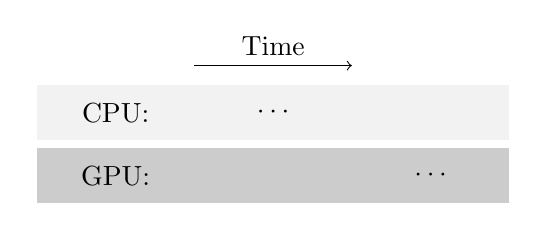
\begin{tikzpicture}
			\draw[->] (-1, 1) -- (1, 1) node [midway, above] {Time};
			\matrix (timeline) [timeline] {
				\node [minimum width=2cm] {CPU:}; \& \cputimeline ; \node {$\cdots$}; \& \noexpand\node{}; \\
				\node [minimum width=2cm] {GPU:}; \& \noexpand\node{}; \& \gputimeline; \node {$\cdots$}; \\
			};
		\end{tikzpicture}
		\subcaption{Execution time line for two frames in flight.}
	\end{subfigure}
	\undef\cputimeline
	\undef\gputimeline
	\caption{Execution time lines for different frames in flight  for the best
	case scenario, i.e.~CPU and GPU requiring the same time for each frame. We
	can see how, when using more than one frame in flight, the CPU can start
	working on the next step of simulation without waiting for the previous one
	to finish. The GPU, in turn, when it finishes the work associated with a
	frame, can start working immediately on the next as the CPU has already
	updated the scene.}
	\label{fig:timeline-optimal}
\end{figure}

\begin{figure}\centering
	\let\cputimeline=\empty
	\foreach \x in {1,...,4} {
		\xappto{\cputimeline}{
			\noexpand\node [draw, fill=green!30, minimum width=.5cm] {\x}; \& \noexpand\node {}; \&
		}
	}
	\let\gputimeline=\empty
	\foreach \x in {1,...,4} {
		\xappto{\gputimeline}{
			\noexpand\node[minimum width=.5cm]{}; \& \noexpand\node [draw, fill=blue!30] {\x}; \&
		}
	}
	\begin{subfigure}[t]{\textwidth}\centering
		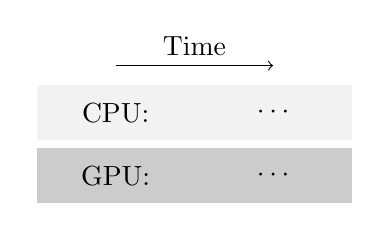
\begin{tikzpicture}
			\draw[->] (-1, 1) -- (1, 1) node [midway, above] {Time};
			\matrix (timeline) [timeline] {
				\node {CPU:}; \& \cputimeline ; \node {$\cdots$}; \\
				\node {GPU:}; \& \gputimeline ; \node {$\cdots$}; \\
			};
		\end{tikzpicture}
		\subcaption{Execution time line for one frame in flight.}
	\end{subfigure}
	\undef\cputimeline
	\undef\gputimeline

	\let\cputimeline=\empty
	\foreach \x in {1,...,5} {
		\xappto{\cputimeline}{
			\if\x1
				\noexpand\node [draw, fill=green!30, minimum width=.5cm] {\x}; \&
			\else
				\noexpand\node [minimum width=2cm]{}; \noexpand\node [draw, fill=green!30, minimum width=.5cm] {\x}; \&
			\fi
		}
	}
	\let\gputimeline=\empty
	\foreach \x in {1,...,5} {
		\xappto{\gputimeline}{
			\noexpand\node [draw, fill=blue!30, minimum width=2cm] {\x}; \&
		}
	}
	\begin{subfigure}[t]{\textwidth}\centering
		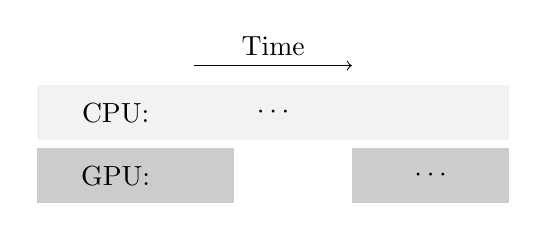
\begin{tikzpicture}
			\draw[->] (-1, 1) -- (1, 1) node [midway, above] {Time};
			\matrix (timeline) [timeline] {
				\node [minimum width=2cm] {CPU:}; \& \cputimeline ; \node {$\cdots$}; \& \node{}; \\
				\node [minimum width=2cm] {GPU:}; \& \node [minimum width=.5cm]{}; \& \gputimeline; \node {$\cdots$}; \\
			};
		\end{tikzpicture}
		\subcaption{Execution time line for two frames in flight.}
	\end{subfigure}
	\undef\cputimeline
	\undef\gputimeline
	\caption{Execution time lines for different frames in flight when the CPU
	time for each frame is significantly less than the GPU time. Using two
	frames in flight still improves the overall throughput but the effect is
	less dramatic than the optimal case pictured in \autoref{fig:timeline-optimal}.}
	\label{fig:timeline-suboptimal}
\end{figure}

As already mentioned, the work performed by the GPU consists first of the ray
tracing which simulates the propagation of the EM waves transmitted by the
radar and then of a transfer operation, which copies back to the host memory
the data associated with the received rays. So far, we have only discussed the
possibility of overlapping the work performed by the CPU with the one performed
by the GPU. However, it is also possible to overlap data transfers and ray
tracing done by the GPU. This, in Vulkan, is achieved by using the dedicated
transfer queue, a queue which supports only transfer operations, which allows
the device to perform \emph{direct memory access} (DMA) to the host memory
\cite{vulkan-queues}. In turn, this means that the data transfer can overlap
freely with independent computations. In our case, the ray tracing for the next
step can start immediately, without waiting for the data transfer of the
previous frame to finish. \autoref{fig:transfer-queue-timeline} shows the
execution timelines for CPU and GPU with a dedicated transfer queue. Since not
all combinations of GPUs and drivers implement a dedicated transfer queue, our
implementation, in case this queue it is not present, gracefully falls back
to perform data transfer on a compute queue.


\begin{figure}\centering
	\def\cputime{.7cm}
	\def\computetime{1.5cm}
	\def\transfertime{.5cm}
	\let\cputimeline=\empty
	\foreach \x in {1,...,5} {
		\xappto{\cputimeline}{
			\if\x1
				\noexpand\node [draw, fill=green!30, minimum width=\cputime] {\x}; \&
			\else
				\noexpand\node [minimum width=\computetime]{}; \noexpand\node [draw, fill=green!30, minimum width=\cputime] {\x}; \&
			\fi
		}
	}
	\let\computetimeline=\empty
	\foreach \x in {1,...,5} {
		\xappto{\computetimeline}{
			\noexpand\node [draw, fill=blue!30, minimum width=\computetime] {\x}; \&
		}
	}
	\let\transfertimeline=\empty
	\foreach \x in {1,...,5} {
		\xappto{\transfertimeline} {
			\noexpand\node [minimum width=\computetime]{}; \noexpand\node [draw, fill=red!20, minimum width=\transfertime] {\x}; \&
		}
	}
	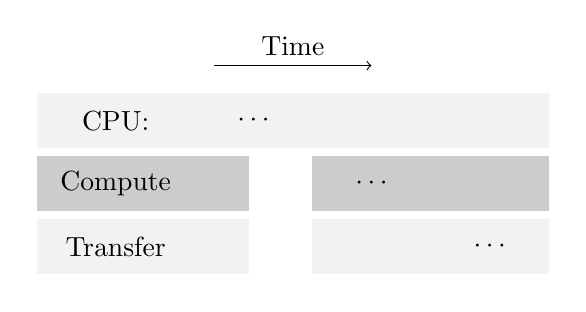
\begin{tikzpicture}
		\draw[->] (-1, 1.5) -- (1, 1.5) node [midway, above] {Time};
		\matrix (timeline) [timeline, nodes={minimum width=\computetime},] {
			\node [minimum width=2cm] {CPU:}; \& \cputimeline ; \node {$\cdots$}; \& \node{}; \& \node{}; \\
			\node [minimum width=2cm] {Compute}; \& \node [minimum width=\cputime]{}; \& \computetimeline; \node {$\cdots$}; \& \node {}; \\
			\node [minimum width=2cm] {Transfer}; \& \node [minimum width=\cputime]{}; \& \node{}; \& \transfertimeline; \node {$\cdots$}; \\
		};
	\end{tikzpicture}
	\undef\cputimeline
	\undef\computetimeline
	\caption{Execution time line when using both two frames in flight and the
	dedicated transfer queue to maximize throughput and keep both the CPU and
	GPU as utilized as possible. The compute timeline refers to a Vulkan queue
	of type compute used for the ray tracing, while transfer refers to a
	transfer-only queue used to transfer efficiently the results of the ray
	tracing to the host.}
	\label{fig:transfer-queue-timeline}
\end{figure}


